% !TeX program = pdfLaTeX
\documentclass[12pt]{article}
\usepackage{amsmath}
\usepackage{graphicx,psfrag,epsf}
\usepackage{enumerate}
\usepackage{natbib}
\usepackage{textcomp}
\usepackage[hyphens]{url} % not crucial - just used below for the URL
\usepackage{hyperref}
\providecommand{\tightlist}{%
  \setlength{\itemsep}{0pt}\setlength{\parskip}{0pt}}

%\pdfminorversion=4
% NOTE: To produce blinded version, replace "0" with "1" below.
\newcommand{\blind}{0}

% DON'T change margins - should be 1 inch all around.
\addtolength{\oddsidemargin}{-.5in}%
\addtolength{\evensidemargin}{-.5in}%
\addtolength{\textwidth}{1in}%
\addtolength{\textheight}{1.3in}%
\addtolength{\topmargin}{-.8in}%

%% load any required packages here




\usepackage{booktabs}
\usepackage{longtable}
\usepackage{array}
\usepackage{multirow}
\usepackage{wrapfig}
\usepackage{float}
\usepackage{colortbl}
\usepackage{pdflscape}
\usepackage{tabu}
\usepackage{threeparttable}
\usepackage{threeparttablex}
\usepackage[normalem]{ulem}
\usepackage{makecell}
\usepackage{booktabs}
\usepackage{longtable}
\usepackage{array}
\usepackage{multirow}
\usepackage{wrapfig}
\usepackage{float}
\usepackage{colortbl}
\usepackage{pdflscape}
\usepackage{tabu}
\usepackage{threeparttable}
\usepackage{threeparttablex}
\usepackage[normalem]{ulem}
\usepackage{makecell}
\usepackage{xcolor}

\begin{document}


\def\spacingset#1{\renewcommand{\baselinestretch}%
{#1}\small\normalsize} \spacingset{1}


%%%%%%%%%%%%%%%%%%%%%%%%%%%%%%%%%%%%%%%%%%%%%%%%%%%%%%%%%%%%%%%%%%%%%%%%%%%%%%

\if0\blind
{
  \title{\bf Causal Inference in Population Trends: Searching for
Demographic Anomalies in Big Data}

  \author{
        Mathew E. Hauer \thanks{Thanks y'all!} \\
    Department of Sociology, Florida State University\\
     and \\     Stephanie A. Bohon \\
    Department of Sociology, University of Tennessee - Knoxville\\
      }
  \maketitle
} \fi

\if1\blind
{
  \bigskip
  \bigskip
  \bigskip
  \begin{center}
    {\LARGE\bf Causal Inference in Population Trends: Searching for
Demographic Anomalies in Big Data}
  \end{center}
  \medskip
} \fi

\bigskip
\begin{abstract}
The proliferation of big data, wider access to advanced computing
platforms, and the development of powerful statistical algorithms can
uncover hidden anomalies in social data, previously dismissed as noise.
Here, we combine causal inference techniques and abductive reasoning to
identify fertility and mortality anomalies on twenty years of
demographic data in the United States. We uncover real, ``hidden'' baby
booms/busts and mortality spikes/dips, distinguishable from regular
trend variations. We identify more than 22 and 156 fertility and
mortality anomalies, totaling more than 200k and 600k anomalous births
and deaths, respectively. Notable detectable mortality anomalies include
the September 11 2001 terrorist attack in New York, the emergence and
acceleration of the opioid epidemic in New Hampshire, and the excess
mortality due to Hurricane Maria in Puerto Rico. Notable fertility
anomalies include the ``missing births'' in Louisiana after Hurricane
Katrina and the reduction in fertility behavior after the September 2008
stock market crash in Connecticut, amongst others. Our combined causal
inference and abductive reasoning approach can be readily adapted to
find other, undiscovered social phenomena or to evaluate the efficacy of
important public policies.
\end{abstract}

\noindent%
{\it Keywords:} mortality, fertility, causal inference, abductive
reasoning, big data
\vfill

\newpage
\spacingset{1.45} % DON'T change the spacing!

\newpage

\hypertarget{introduction}{%
\section{Introduction}\label{introduction}}

The search for causality is one of the primary motiviations behind
social science \citep{smith2011commentary, pearl2009causal}. Causal
Inference, the identification of causal mechanisms, attempts to uncover
the underlying mechanisms that result in changes in a phenomenon and has
a long history as an approach to inquiry in the social sciences
\citep{grimmer2015ppsp}. Often, the identification of a casual mechanism
is accomplished via a randomized control trial (RCT) or expert knowledge
applied to a natural experiment \citep{salganik2019bit}.

Unfortunately, both RCTs and natural experiments have drawbacks. RCTs
are often prehibitively expensive for many scientists, precluding their
widespread adoption in the social sciences \citep{west2008ajph}. RCTs
are also sometimes impossible to deploy in the ``real world''. For
instance, an RCT to study country-level austeriy measures would be
difficult, if not impossible, to implement. Natural experiments are a
cheaper alternative, but provide less certainty about causation, fewer
opportunities to replicate work, and require expert knowledge of the
natural experiment to be properly employed \citep{pearl2018book}.

Additionally, both RCTs and natural experiments follow traditional
hypothesis testing, the deductive scientific paradigm where a question
is first posed and scientists generate or find data to answer the
question. Such approaches, while extensively utilized and time-tested,
are likely to miss important phenomena that might go unnoticed or suffer
from extensive p-hacking
\citep{head2015extent, nuzzo2014scientific, ruggles2014big}. Abductive
reasoning, sometimes described as ``inferring cause from effect''
\citep{Crowder2017}, moves the scientific process from the inductive to
the deductive, and sometimes back and forth, to reach conclusions
\citep{bryant2014realm} The physical sciences use abductive reasoning
more fully compared to the social sciences. The discovery of Neptune in
1846 based on unexplained perturbations of the orbit of Uranus
\citep{popper2005logic}, the discovery of galactic migration of planets
\citep{gomes2005n}, and the current generation of gravitational wave
detectors such as the Laser Interferometer Gravitational-Wave
Observatory (LIGO) \citep{harry2010advanced} demonstrate the power of
the abductive approach in the physical sciences.

In a data-rich environment, abductive reasoning can be more easily
applied to first find effects and then infer their cause ex-post. The
modern proliferation of data, advances in high performance (``super'')
computing, and the development of powerful statistical algorithms
provide an environment ripe for wedding causal inference with abductive
reasoning \citep{van2016data, zikopoulos2011}, with the potential for
researchers to find hidden or understudied social phenomena
\citep{bohon2018demography}. While the availability of Big Data and high
performance computing allows novel exploration of data through causal
inference
\citep{bohon2018demography, rcausalimpact, shiffrin2016drawing},
relatively few studies utilize causal inference techniques in the study
of demographic phenomena. However, understanding social phenomena using
these advances reveals important insights into society
\citep{angrist1989lifetime, mas2009peers} and allows us to better
monitor population trends \citep{nobles2019, torche2015hidden}. The rich
demographic data available in the United States make the potential
revelation of interesting and important demographic phenomena not only
possible, but extremely plausible -- even if identification of the
phenomena occurs without identifying the underlying cause.

In this paper, we combine a modern statistical outlier detection
algorithm \citep{chen1993joint}, abductive reasoning, and large
demographic data sets on more than 20 years of mortality/fertility to
identify anomalous demographic behavior. In essence, we identify
\emph{effects without knowledge of the cause}. We ask one fundamanetal
question regarding demographic anomalies: What are the hidden baby
booms/busts and mortality spikes/dips in the United States over the last
twenty years? We do not necessarily know the causes of these anomalies
but identifying them allows scientists with more detailed knowledge of
local population dynamics, state-level policy making, or macro-economics
to explain these phenomena post-hoc. From explanations of phenomena that
may have previously gone unnoticed, social scientists may be able to
better forecast populations and provide policy solutions for impending
problems such as climate change.

\hypertarget{materials-and-methods}{%
\section{Materials and Methods}\label{materials-and-methods}}

\hypertarget{method}{%
\subsection{Method}\label{method}}

We use a statistical time series outlier detection algorithm
\citep{chen1993joint}, implemented in the R programming language
\citep{rcore} via the tsoutliers package \citep{tsoutliers2019}. This
algorithm iteratively uses ARIMA models to 1) produce a counter-factual
time series to initially detect an outlier or anomaly, and 2) refit the
ARIMA with the outliers removed. Here we briefly summarize and describe
the method.

Often, the behavior of a time series can be described and summarized in
ARIMA models. If a series of values, \(y_t^*\), is subject to \(m\)
interventions or outliers at time points \(t_1,t_2,…,t_m\), then
\(y_t^*\) can be defined as

\[y_t^* = \sum_{j=1}^{m} \omega_jL_j(B)I_t(t_j) + \frac{\theta(B)}{\phi(B)\alpha(B)}\alpha_t\]

Where \(I_t(t_j)\) is an indicator variable with a value of 1 at
observation \(t_j\) and where the \(j\)th outlier arises, \(\phi(B)\) is
an autoregressive polynomial with all roots outside the unit circle,
\(\theta(B)\) is a moving average polynomial with all roots outside the
unit circle, and \(\alpha(B)\) is an autoregressive polynomial with all
roots on the unit circle.

We examine three types of outliers at time point \(t_m\): 1) additive
outliers (AO), defined as \(L_j(B)=1\); 2) level shift outliers (LS),
defined as \(L_j(B) = 1/(1-B)\); and 2) temporary change outliers (TC),
defined as \(L_j(B) = 1/(1-\delta B)\).

Colloquially, additive outliers arise when a single event causes the
time series to unexpectedly increase/decrease for a single time period;
level shift outliers arise when an event causes the time series to
unexpectedly increase/decrease for multiple time periods; and temporary
change outliers arise when an event causes the time series to
unexpectedly increase/decrease with lingering effects that decay over
multiple time periods.

An outlier is detected using a regression equation

\[ \pi(B)y_t^* \equiv \hat{e} = \sum_{j=1}^m \omega_j \pi(B)L_j(B)I_t(t_j) + \alpha_t \]

\begin{figure}
\centering
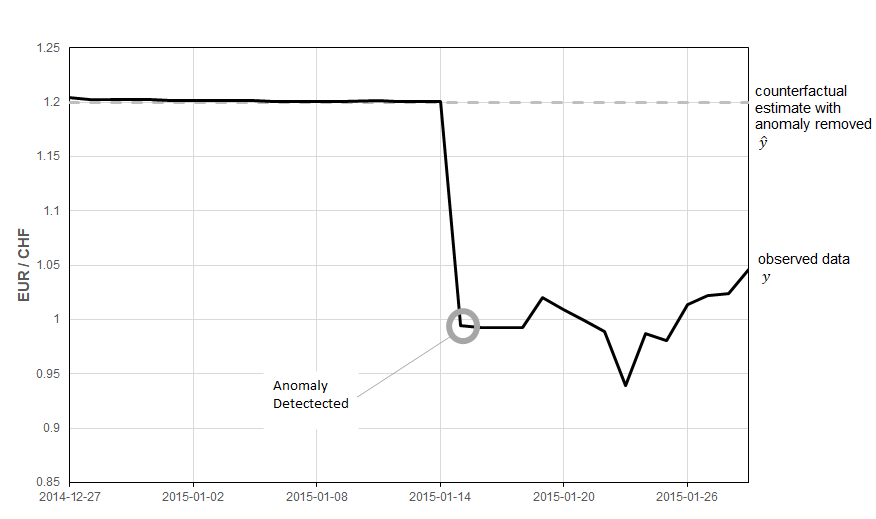
\includegraphics{./manuscript_files/figure-latex/Figure1.png}
\caption{\textbf{``Toy'' example of anomaly detection using the exchange
rate between the Euro and the Swiss Franc.} The Swiss Franc was pegged
to the Euro at 1.2 until January 15 2015 when the peg was removed and
the currency was allowed to trade more freely. This is a very strong
anomly in the time series (\emph{t}-stat = -144.07) detectable using
statistical methods and visually. The countefactural estimate with the
outlier removed would simply have kept the currency exchange at 1.2
(\(\hat{y}\)). \label{explanationfigure}}
\end{figure}

where \(\pi(B)=\sum_{i=o}^{inf} \pi_iB^i\). The identification of
outliers then involves a three step process. First, (1) the algorithm
identifies all potential outliers, \(t_j\) and \(L_j (B)\). Next, (2) we
compute joint estimates of model parameters and outlier effects to
identify potentially spurious outliers. Finally, (3) the outliers and
effects are re-estimated without spurious outliers. Of importance here
is step 2, which relies on some critical value above which an outlier at
time point \(m\) is considered spurious. Based on Chen and Liu's
\citeyearpar{chen1993joint} recommendation, we set a critical value of
3.5 which generally minimizes the possibility of Type I errors or false
positive outliers.

We report outliers using a simple t-statistic and report the size of the
outlier, or its impact on the time series, by subtracting \(\hat{y}\),
the adjusted time series with outliers removed, from \(y\), the
original, unadjusted time series.

\textbf{\autoref{explanationfigure}} shows a toy example for anomaly
detection in a time series using the classic example of the exchange
rate between the Euro and the Swiss Franc (CHF). On January 15 2015, the
Swiss National Bank removed the currency peg of 1.20 francs per Euro,
exposing the Franc to the volatility of the currency market. The Franc
immediately began trading a reduced rate compared to the Euro. What
would have been the Euro/CHF exchange rate had the Swiss National Bank
\emph{not} removed the peg? A simple counter-factual estimate would be
to keep the exchange rate at 1.20 (\(\hat{y}\), sometimes called a
``synthetic control'' \citep{abadie2010synthetic}).

In the Swiss Franc example, we have knowledge of the Swiss Bank's
activities after the fact or ex-post-facto to to create the
counter-factual time series \(\hat{y}\) of 1.20. But is this anomaly
detectable without knowledge of the Swiss Bank's activities? In other
words, can we detect the reduction of the exchange rate on January 15
using only the time series? Absolutely. the tsoutliers package
identifies January 15 2015 as an extremely strong level-shift outlier
(\emph{t}-stat = -144.07). The real world is hardly this simplified
where a direct intervention is known and is testable.

\hypertarget{data}{%
\subsection{Data}\label{data}}

We search for demographic anomalies using the Center for Disease Control
and Prevention's online WONDER monthly fertility (2003-2017) and
mortality databases (1999-2016) for all fifty states and the District of
Columbia \citep{CDC_fert07, CDC_mort}. These data sets contain every
birth and death record in the United States over the time periods of
interest, representing the universe of both mortality and fertility data
in the US. These data are considered the ``gold standard'' of data
collections \citep{mahapatra2007civil} and have been considered
``complete'' since 1968 \citep{hetzel2016us}. We search over each state
equivalent's (n=51) mortality (n=228) and fertility (n=180) monthly time
series for a total of 20,808 state-months of data.

\hypertarget{results}{%
\section{Results}\label{results}}

We detect numerous anomalous mortality and fertility events at the US
state-level since 1999. A full listing of these anomalies can be found
in the \textbf{Supplementary Materials}. We begin by highlighting
significant fertility and mortality anomaloies across all three types of
outliers (Additive Outliers, Level Shift Outliers, and Temporary Change
outliers) with plausible explanations. We then highlight two strong
anomalies that bely explanation. Finally, we conclude with a summary of
the anomalies we detect.

\hypertarget{fertility}{%
\subsection{Fertility}\label{fertility}}

We begin with a clear temporary change (TC) outlier for fertility in
Louisiana (\textbf{\autoref{fig:fertla}a}). Here we detect two TC
outliers, nearly back-to-back in 2005 (2005:08 \emph{t} = -6.002; and
2005:10 \emph{t} = -4.997), coinciding with the destruction of Hurricane
Katrina from the same year. The migration associated with Hurricane
Katrina has garnered most of the attention of social scientists
\citep{fussellRecoveryMigrationCity2014, horiDisplacementDynamicsSouthern2009},
but the hurricane had a very clear impact on fertility behaviors too,
creating a mini ``baby bust'' in Louisiana with the departure of many
people in their childbearing years. We estimate 4,411 fewer births in
Louisiana compared to the counterfactual, likely attributable to the
Hurricane.

We also highlight a level shift (LS) outlier for fertility in
Connecticut. Here we detect a strong (\emph{t}= -3.71 for -285
births/month) level shift toward lower fertility beginning in August
2009 (2009:08) that continues through the end of the period
(\textbf{\autoref{fig:fertla}b}). This LS toward lower fertility reduced
the number of births by 28,752 or 9\%) lower than the counterfactual
time series. The stock market crash of 2008, where the Dow Jones
Industrial Average had the largest single-day loss up to that point,
occurred just 11 months before we detect a shift toward lower fertility.
It is possible that the trend toward lower fertility in August 2009 and
the stock market crash in September 2008 are linked, although, as stated
previously, we are speculating only to illustrate how causal inference
could work in an abductive research agenda. A potentially interesting
future line of research would be to link fertility anomalies to the
kinds of economic shocks that may lead to outmigration of those in their
childbearing years.

\begin{figure}
\centering
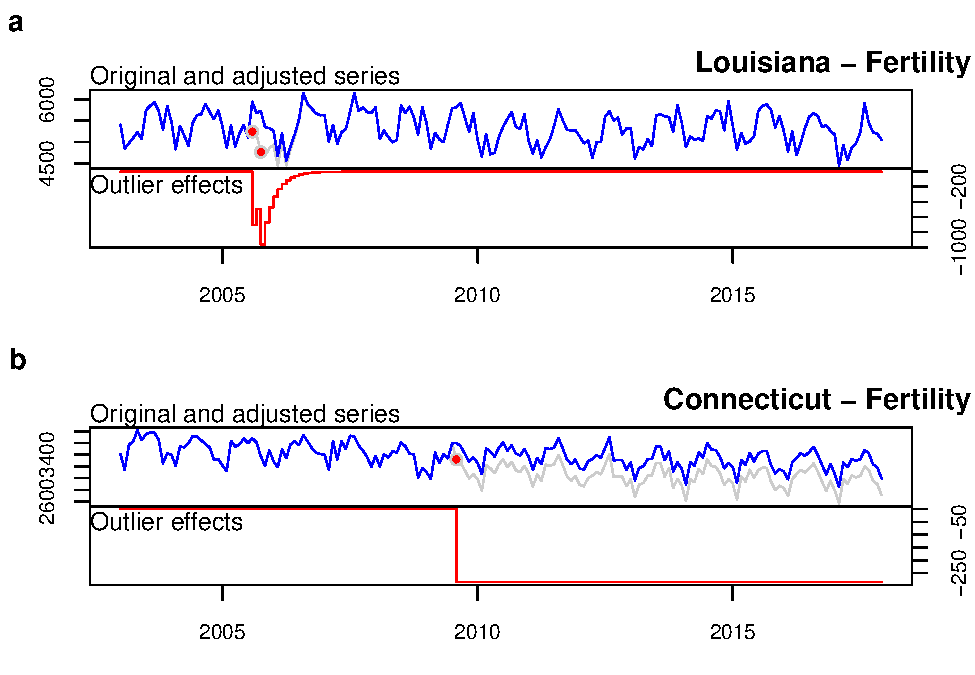
\includegraphics{manuscript_files/figure-latex/FertilityAnomalies-1.pdf}
\caption{\textbf{Anomaly detection in Louisiana (a) and Connecticut (b) state fertility, 2003-2018.}
The top part of each panel contains the original time series (light
gray), the corrected, counter-factual time series in the absence of
anomalies (blue), and the red dots correspond to the onset of detected
anomalies. The bottom part of each panel contains the magnitude and type
of the outlier in red. In (a), we detect two outliers, back-to-back,
likely resulting from Hurricane Katrina in August and October 2005,
representing a decrease of more than 4,400 births due to the hurricane
(t-statistics= -6.002 and -4.997). In (b), we detect one outlier, a
level shift outlier (LS) in August 2009. We believe this reduction is
attributable to the stock market crash 11 months earlier (t-statistic =
-3.71). \label{fig:fertla}}
\end{figure}

\hypertarget{mortality}{%
\subsection{Mortality}\label{mortality}}

For mortality, we will use New York State as an example
(\textbf{\autoref{fig:mortnewhamp}a}). We identify seven anomalies in
the mortality time series for New York, all with \emph{t}-statistics in
excess of 3.91, making these anomalies unlikely to be due to chance. The
algorithm correctly identifies September 2001 as an additive outlier
(2001:09 \emph{t}= 6.396) where there were 1,628 more deaths in that
month than anticipated. This mortality event is likely caused by the
September 11 terrorist attack on the World Trade Center that immediately
killed 2,606 people and the detection of this mortality event provides
confidence in our detection of other anomalies.

In \textbf{\autoref{fig:mortnewhamp}a}, notice the strong level shift
(LS) that occurs in February 2004 (2004:02 \emph{t}= -5.594) which
prevented 869 deaths per month. This shift totals more than 144,000
averted deaths compared to the counter-factual time series and is the
single largest mortality protective anomaly among all states. This
translates to 7\% fewer deaths than expected over the time period. What
is driving this mortality protection? What policies did NY put into
place that might have contributed to this considerable mortality
reduction? What environmental or economic conditions may have changed
may have changed? These are the kinds of questions that arise from our
analyses. The purpose of our paper is not to answer these questions, but
our findings underscore the need for more research that takes an
abductive approach. By identifying anomalies through an inductive
process, researchers can then look for underlying causes. Once those
causes are identified, researchers can then use a deductive process to
see if such events predict other (or future) anomalies.

To see the potential for combining abductive reasoning with causal
inference, contrast the mortality protection in New York with the
enhanced mortality in New Hampshire
(\textbf{\autoref{fig:mortnewhamp}b}). In New Hampshire we detect two
significant level shifts (LS) in the monthly mortality data, first in
April 2010 and again in November 2014 (2010:04 \emph{t}= 3.51; 2014:11
\emph{t}= 6.68). These anomalies suggest New Hampshire experienced 8,159
more deaths (+9\% more than expected) in a seven-year period beginning
in early 2010. These are events not experienced by neighboring states
during the same time period, and this is the single largest percentage
mortality increase/decrease we detected among all states. Not
coincidentally, NH has the second highest opioid-related mortality in
the US \citep{beetham2019access} and it is likely that we detect this
epidemic in our results. Isolating these anomalies and testing them
against opioid sales data might yield intriguing results.

\begin{figure}
\centering
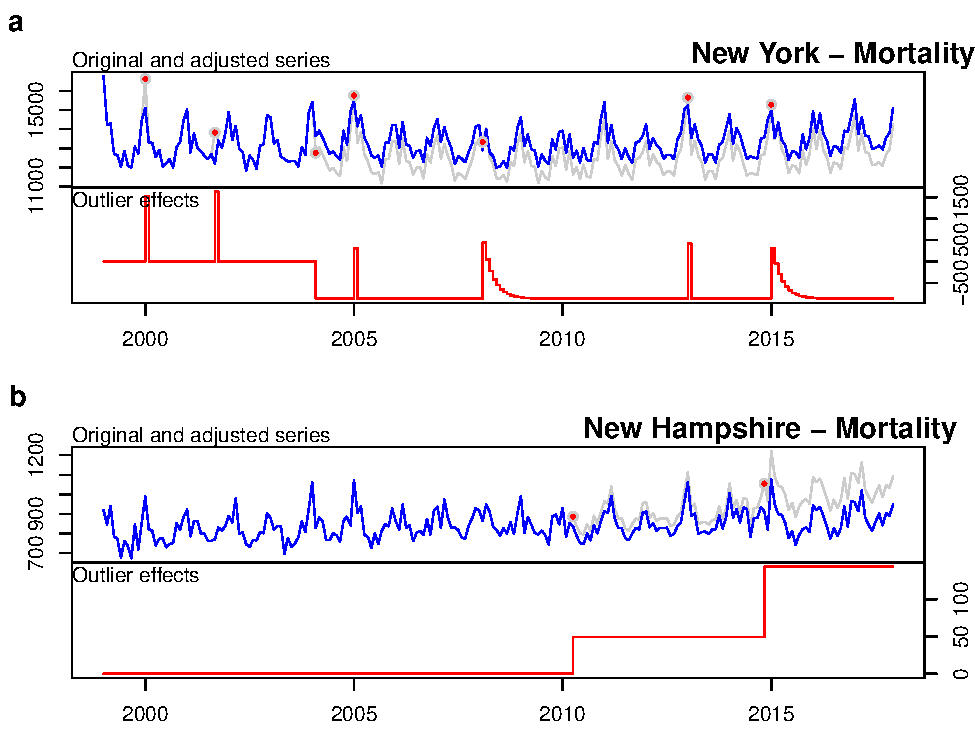
\includegraphics{manuscript_files/figure-latex/MortalityAnomalies-1.pdf}
\caption{\textbf{Anomaly Detection for New York (a) and New Hampshire (b) state mortality, 1999-2016.}
In New York (a), we detect additive outliers (AO) in January 2000,
September 2001, January 2005, and January 2013; temporary change (TC)
outliers in February 2007 and January 2015; and a level shift (LS)
starting in February 2004. In New Hampshire (b), we detect two outliers,
both level shift outliers (LS) in April 2010 and again in November 2014.
These anomalies suggest New York experienced a significant mortality
event in September 2001 and New Hampshire experienced approximately
9,700 more deaths than expected since 2010 or 14\% more deaths in the
state over just seven years. \label{fig:mortnewhamp}}
\end{figure}

\hypertarget{interesting-anomalous-fertilitymortality-events}{%
\subsection{Interesting Anomalous Fertility/Mortality
events}\label{interesting-anomalous-fertilitymortality-events}}

In the examples above, we highlighted four fertility/mortality anomalies
with plausible explanations. In the case of New York and New Hampshire,
the mortality anomalies have plausible explanations. It seems likely
that New York's AO anomaly in September 2001 is caused by the 9/11
tragedy and the rise in New Hampshire's mortality starting in 2010 could
be linked to the opioid epidemic. Similarly, Louisiana's TC anomalies
seem linked to Hurricanes Katrina and Rita while the LS anomaly in
Connecticut's fertility appears linked to the Great Recession. However,
we detect numerous other demographic anomalies in other states, on the
causes of which we will not speculate. \textbf{\autoref{fig:ferthawaii}}
shows two such unexplained anomalies.

In \textbf{\autoref{fig:ferthawaii}a} we identify a single additive
anomaly in Hawaiian fertility in May 2014. This is a strong anomaly with
a \emph{t}-statistic of 4.96, 15\% above the counter-factual time
series. This single, anomalous month is also the second highest monthly
births in the time series. We have no plausible explanation for this
anomaly. We do not believe this is simply a data error as the other
extreme values, September 2008 and February 2005 with the highest and
lowest recorded fertility respectively, were not identified as anomalous
events. Even if we were to assume this anomaly resulted from data entry
error, it remains an \emph{unaltered} data error in the Hawaiian monthly
fertility data.

This is contrast to \textbf{\autoref{fig:ferthawaii}b}, where we
identify a strange mortality reduction in Ohio (\emph{t}-stat: -4.27).
This LS is more than 1,157 deaths per month less than the counterfactual
time series, suggesting had nearly 40,000 fewer deaths since February
2015 than expected. This is the single-largest LS among all states. We
could not identify the potential policies Ohio might have put into place
to provide such a strong mortality protection.

\begin{figure}
\centering
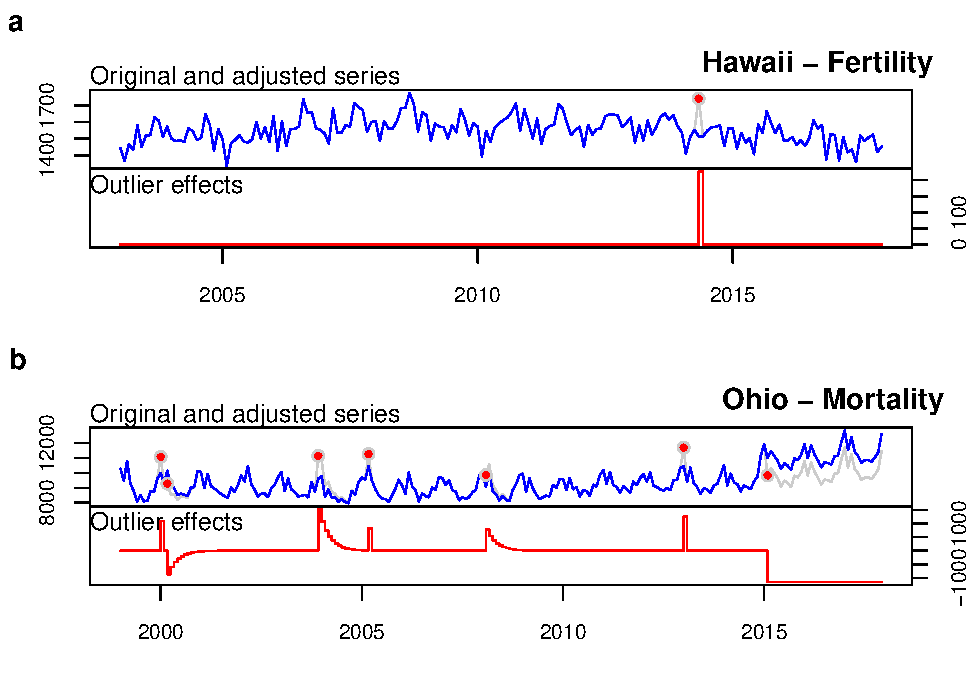
\includegraphics{manuscript_files/figure-latex/TrueAnomalies-1.pdf}
\caption{\textbf{Anomaly detection in Hawaii state fertility (a) and Ohio state mortality (b).}
Here we detect one outlier, an additive outlier (AO) in May 2014 in
Hawaii (a), representing a large, unexplainable 14\% increase in
expected births in that month. We also detect a strong level shift (LS)
reduction (b), representing a large, unexplainable reduction of nearly
40,000 deaths in Ohio. \label{fig:ferthawaii}}
\end{figure}

\hypertarget{overall-anomalies}{%
\subsection{Overall Anomalies}\label{overall-anomalies}}

\begin{table}

\caption{\label{tab:unnamed-chunk-6}\textbf{Summary by Demographic Component.}  Here we can see there 22 Fertility and 156 Mortality anomalies among the state-level time series, totalling more than 200k anomalous births and 600k anomalous deaths. \label{sumtable}}
\centering
\begin{tabular}[t]{lrllrrr}
\toprule
Component & Anomalies & $y$ & $\hat{y}$ & $y-\hat{y}$ & $|y-\hat{y}|$ & \% of Total\\
\midrule
Fertility & 22 & 25.48M & 25.68M & -202,217 & 226,476 & 0.889\\
Mortality & 156 & 43.57M & 43.52M & 48,535 & 627,364 & 1.440\\
\bottomrule
\end{tabular}
\end{table}

\textbf{\autoref{sumtable}} reports the overall number of anomalies we
detect of each type for births and deaths and some summary statistics
across all anomaly types and \textbf{\autoref{fig:summap}} maps these
results.

We find considerably more mortality anomalies (n = 156) than fertility
anomalies (n = 22). Given that anomalies are always the product of
events \citep{song2018anomaly}, finding more mortality than fertility
anomalies is not surprising. Mortality is likely to spike in response to
a catastrophic event (like an earthquake or terrorist attack) or due to
a disease outbreak while the effects of a catastrophic event on
fertility is less predictable. One reason for this is that fertility is
linked to human decision-making more directly than mortality
\citep{stein2014couples} which results in more varied outcomes, so, for
example, researchers find that catastrophic weather events can increase
childbearing among those who already have a child, but not among the
childless \citep{Evans2008Hurricanebirth}. Some events, like the 1995
Oklahoma City bombings, resulted in both fertility and mortality
changes. However, changes in fertility manifest over a longer time
horizon after an event, and the relationship between a
fertility-inducing event and behavior change is less strong than the
relationship between a mortality-inducing event (such as a terrorist
incident) and death \citep{Rodgers2005OKBombing}. Of course, not all
events that impact fertility and mortality are catastrophic. Researchers
have documented that more commonplace events such as massive layoffs
\citep{Venkataramani2019} or policy changes
\citep{Livingston2017Cannabis} can also create anomalies in mortality
patterns, but we have not found such evidence for fertility.

Consistent with more anomalies across the time series, we find more
anomalous deaths (627,364) than anomalous births (226,476). Fertility
anomalies overwhelmingly tend toward lower fertility, with only a few
fertility anomalies yielding more births. This is consistent with
research findings that link high severity weather events to
significantly lower fertility \citep{Evans2008Hurricanebirth}.
Conversely, mortality anomalies tend to be more evenly split between
positive and negative anomalies, but tend toward more deaths rather than
fewer deaths. Again, this is not surprising, as the kinds of events that
increase death (e.g., plant closings are associated with increased
opioid death \citep{Venkataramani2019}) are more common than the events
that decrease death (e.g., cannabis legalization is associated with
decreased opioid deaths \citep{Livingston2017Cannabis}). These anomalous
deaths and births account for 1.44\% and 0.889\% over the entire time
series, respectively.

As \textbf{\autoref{fig:summap}} shows, three states exhibited neither
mortality nor fertility anomalies: Alaska, North Dakota, and South
Dakota. Another nine states exhibited just a single anomaly (DE, DC, ID,
IL, KS, NV, NM, UT, and WY). Both New York and Massachusetts exhibited
the most anomalies with nine.

\begin{figure}
\centering
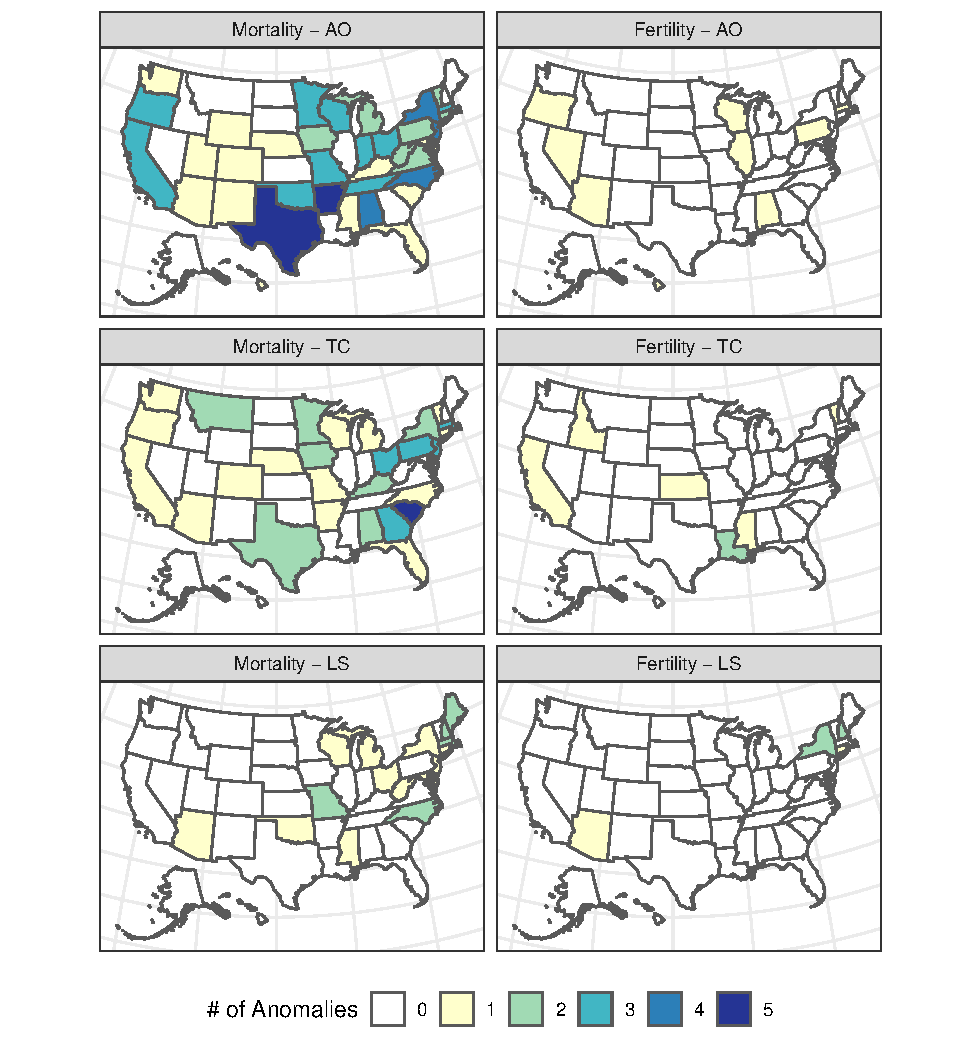
\includegraphics{manuscript_files/figure-latex/AnomalyMap-1.pdf}
\caption{\textbf{Summary of Anomalies by type, demographic component, and State.}
We observe much fewer fertility anomalies than mortality anomalies.
\label{fig:summap}}
\end{figure}

\hypertarget{conclusion}{%
\section{Conclusion}\label{conclusion}}

Data scientists frequently claim that the big data revolution is a
turning point in scientific discovery that will allow us to solve some
of the world's most pressing problems \citep{grimmer2015ppsp}. Social
scientists are skeptical of such claims, because they better understand
the complexities of the social world and know from experience that data
alone is not enough to solve social problems
\citep{bohon2018demography, grimmer2015ppsp}. Nonetheless, the increased
availability of data and (more importantly, we argue) the development of
advanced techniques for analyzing these data will enable important
discovery \citep{monroe2015no}.

One technique that population scientists underutilize is causal
inference. Causal inference, in the simplest terms, is the discovery of
effects in search of a cause using big data and advanced computing
algorithms \citep{imai2008misunderstandings}. This inductive approach is
uncommon in quantitative social science where hypothesis testing is
expected, and approaches are largely deductive. However, common
statistical hypothesis testing is impractical with big data, as
significant p values are guaranteed, and such approaches do not allow us
to uncover all the information that big data has to offer
\citep{monroe2015no}. Here, we call for an abductive approach, where
causal inference algorithms are applied to high quality data to uncover
irregularities that are unlikely to be attributable to expected
variations in trends (or noise) as a first step to then developing
testable hypotheses about causes. Abductive approaches allow researchers
to move from the inductive to the deductive and sometimes work back and
forth in aid of scientific discovery.

In this paper, we show how the tsoutlier package in R can be implemented
to conduct statistical time series outlier detection, an inductive
approach that aids in the creation of deductive reasoning. This
algorithm is one of many causal inference approaches that are freely and
commercially available (see \citet{rcausalimpact}). In our initial work,
we experimented with other approaches, such as Google's causalimpact
algorithm, which uncovered the same patterns we briefly discuss in this
paper. By making more use of causal inference techniques and abductive
modeling approaches, we argue that social scientists will be able to
better understand how events or policy implementation can impact
important outcomes. For example, we could uncover---on a wide
scale---how gun control policies may reduce or increase injuries from
shootings or how marijuana legalization might impact opioid deaths. We
could also uncover how increases in extreme weather events impact a
range of behaviors such as home sales, bottled water purchases, and even
fertility.

In our demonstration, we show how the application of causal inference to
state-level time series fertility and mortality data uncovers three
types of demographic anomalies: those that occur and disappear quickly,
those that occur and decay over time, and those that occur and remain.
Uncovering these anomalies in and of themselves is important. For
example, the algorithm we deploy clearly shows the fertility effects of
Hurricanes Katrina and Rita as well as the mortality effects of the
World Trade Center collapse on September 11, 2001. The ability to
identify and differentiate types of anomalies is even more important, as
we can potentially see how some policies might impact outcomes
permanently and some might have an effect that is short-lived.
Differentiating these types gives us greater insight into short- and
long-term solutions to social problems. We urge social scientists to
begin to use causal inference algorithms and other big data techniques,
and we hope that this demonstration will illustrate their usefulness to
the social science enterprise.

\newpage

\bibliographystyle{agsm}
\bibliography{mybibfile}

\end{document}
